
\chapter{Stream Processing Platforms}
\label{chapter:platform}

\begin{figure}
  \begin{center}
  \subfigure{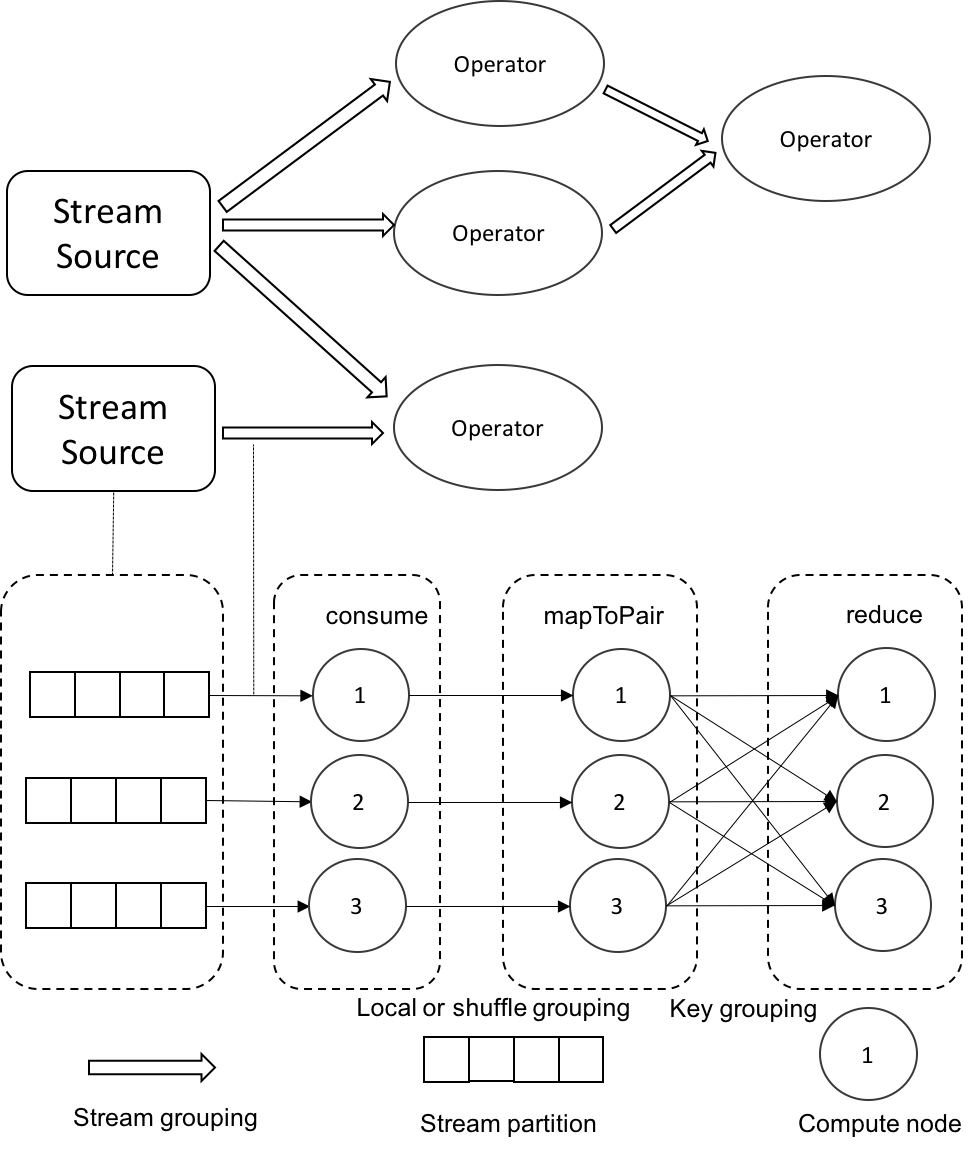
\includegraphics[scale=0.46]{images/stream_process_model}}
   \caption{Stream processing model}
   \label{fig:stream_process_model}
  \end{center}
\end{figure}

There are many stream processing systems that include Apache Apex, Aurora, S4, Storm, Samza, Flink, Spark Streaming, IBM InfoSphere Streams, and Amazon Kinesis. More new stream processing systems are being developed. The design, computational model, and architecture of these systems are different so that they own different features and have different performance. Among these systems, some are not open sourced and it is impossible to download and setup a stream processing cluster. For instance, Amazon Kinesis is only available in AWS. Some ones are open source systems with system design, source code public. That enables us to set up our own distributed cluster to run experiment benchmarks. In StreamBench, we choose three popular and widely used open source stream processing systems which have many similarities. These systems are Storm, Flink, and Spark Streaming. 


First, all these systems are MapReduce inspired, they consider the stream as keyed tuples, support transformations similar to \texttt{Map} and aggregations like \texttt{Reduce}. The computational models of these systems are also similar which are graphs consisted of transformations and/or aggregations. Unlike MapReduce, these systems deal with unbounded stream of tuples and support integration with Kafka, a distributed messaging system discussed in \cref{subsection:kafka}, in which stream data is distributed in different partitions. Moreover, these stream processing frameworks run tasks in parallel. Integrated with distributed message system, these systems achieve both data parallelism and task parallelism of parallel computing. The lower part of Figure~\ref{fig:stream_process_model} shows that 3 compute nodes in a cluster consume messages from a Kafka topic with 3 partitions and run operators \texttt{mapToPair} and \texttt{reduce} in parallel. Each record in the stream is a tuple and there are different ways to forward tuples from a operator to another one, such as key grouping, all grouping, and shuffle grouping.  The computational topology of these systems is a graph shown as the upper part of Figure~\ref{fig:stream_process_model} in which nodes are stream sources and operators connected by stream grouping. Another similarity of these systems is horizontal scalability. Work with these systems, we could add more machines into a stream processing cluster to achieve better performance.

% similarities of all the frameworks

In this chapter, we introduce these three systems in detail from different perspectives: system architecture, computational model, and key features. Several other stream processing systems are also discussed. 
 
\section{Apache Storm}
Apache Storm, one of the oldest distributed stream processing systems which was open sourced by Twitter in 2011 and became Apache top-level project in 2014.  Storm is to realtime data processing as Apache Hadoop is to batch data processing. A Hadoop job is finished after all data processing operations are done. Unlike Hadoop, Storm is an always-active service that receives and processes unbounded streams of data and delivers that data instantaneously, in realtime. Storm solutions can also provide guaranteed processing of data, with the ability to replay data that was not successfully processed the first time.With its simple programming interface, Storm allows application developers to write applications that analyze streams of tuples of data; a tuple may can contain object of any type.

\subsection{Storm Architecture}
\begin{figure}
  \begin{center}
  \subfigure{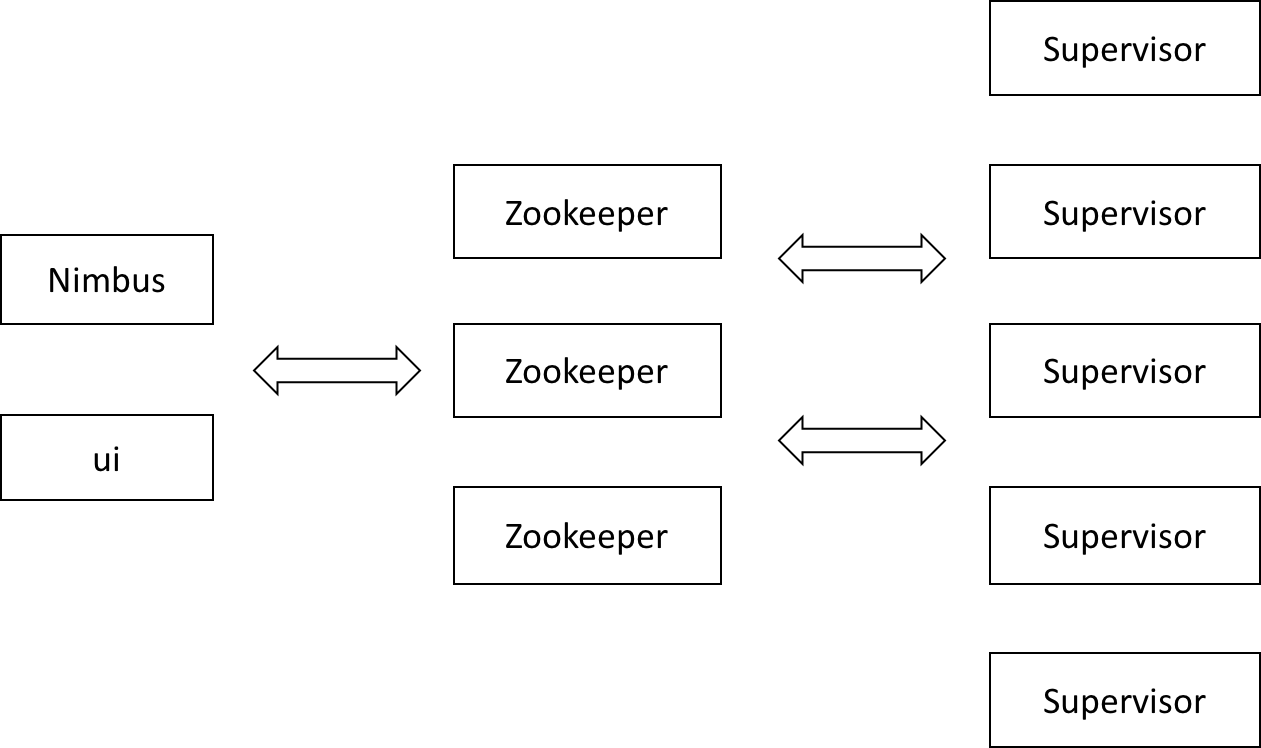
\includegraphics[scale=0.45]{images/storm_cluster}}
   \caption{Storm cluster components}
   \label{fig:storm_cluster}
  \end{center}
\end{figure}

As a distributed stream processing system, a storm cluster consists of a set of nodes. Figure~\ref{fig:storm_cluster} shows components of a storm cluster which contains four different kinds of nodes, ``Supervisor", ``Nimbus", ``Zookeeper" and ``UI". 

Nimbus is a daemon running on the master node which is similar to Hadoop's ``JobTracker". Nimbus is responsible for distributing code around the cluster, assigning tasks to machines, and monitoring for failures. Each worker node runs a daemon called the ``Supervisor". It listens for work assigned to its machine and starts and stops worker processes as dictated by Nimbus. Each worker process executes a subset of a topology; a running topology consists of many worker processes spread across many machines.

All coordination between Nimbus and the Supervisors is done through a Zookeeper cluster. Additionally, the Nimbus daemon and Supervisor daemons are fail-fast and stateless; all state is kept in Zookeeper or on local disk. Hence, Storm clusters are stable and fault-tolerant

UI is a daemon which monitors summary of cluster and running topologies on a web interface. Properties of a topology (such as id, name, status and uptime) and emitted tuples of a spout or bolt also could be found in ``UI". More detail about understanding the Storm UI could be found on the page~\footnote{\url{http://www.malinga.me/reading-and-understanding-the-storm-ui-storm-ui-explained/}}.


\subsection{Computational Model}

The core of Storm data processing is a computational topology, which is a graph of stream transformations similar to the one in Figure~\ref{fig:stream_process_model}. In the computational topology, stream source is consumed by a type of operator called spout. The operator with processing logic is called bolt. Spouts read tuples from external sources (e.g. Twitter API, Kafka) or from disk, and emit them in the topology. Bolt receives input streams from spout or other bolt, process them and produce output streams. They encapsulate the application logic which dictates how tuples are processed, transformed,aggregated, stored, or re-emitted to other nodes in the topology for further processing. When a spout or bolt emits a tuple to a stream, it sends the tuple to every bolt that subscribed to that stream.

A stream in topology is an unbounded sequence of tuples. Spouts read tuples from external sources continuously. Once a topology is submitted, it processes messages forever, or until it is killed. Storm will automatically reassign any failed tasks. Each node in a Storm topology executes in parallel. In your topology, you can specify how much parallelism you want for each node, and then Storm will spawn that number of threads across the cluster to do the execution. 

Additionally, Storm guarantees that there will be no data loss, every tuple will be fully processed at least once. This is achieved by following steps:

\begin{enumerate}
\item Each tuple emitted in a spout is specified with an unique message ID;
\item Each tuple emitted in a bolt, anchor it with corresponding input tuples; 
\item When bolts are done processing the input tuple, ack or fail the input tuple
\end{enumerate}

This mode tracks whether each spout tuple is fully processed within a configured timeout. Any input tuple not fully processed within the timeout is re-emitted. This means the same tuple could be processed more than once and messages can be processed out-of-order. 


\section{Apache Flink}
Apache Flink used to be known as Stratosphere which was started off as an academic open source project in Berlin's Technical University in 2010. Later, it became a part of the Apache Software Foundation incubator and was accepted as an Apache top-level project in December 2014. Apache Flink aims to be a next generation system for big data system. It is a replacement for Hadoop MapReduce that works in both batch and streaming models. Its defining feature is its ability to process streaming data in real time. In Flink, batch processing applications run efficiently as special cases of stream processing applications.

\subsection{Flink Architecture}
The architecture of Flink is a typical master-slave architecture that is quite similar with other scaleable distributed cloud systems. The system consists of a JobManager and one or more TaskManagers. JobManager is the coordinator of the Flink system, while TaskManagers are the workers that execute parts of the parallel programs. 

In Hadoop MapReduce, reduce operation wouldn't start until map operation is finished. In Flink records are forwarded to receiving tasks as soon as they are produced which is called pipelined data transfers. For efficiency, these records are collected in a buffer which is sent over the network once it is full or a certain time threshold is met. This threshold controls the latency of records because it specifies the maximum amount of time that a record will stay in a buffer without being sent to the next task. 

Flink's runtime natively supports both stream and batch processing due to pipelined data transfers between parallel tasks which includes pipelined shuffles. Batch jobs can be optionally executed using blocking data transfers. They are special cases of stream processing applications.

%\subsection{Memory Management}
%One specific feature of Flink is that Flink has its own memory management system. Conceptually, Flink splits the heap into three regions: ~\footnote{\url{https://cwiki.apache.org/confluence/pages/viewpage.action?pageId=53741525}}

%\begin{itemize}
%\item \textbf{Network buffers:} A number of 32 KiByte buffers used by the network stack to buffer records for network transfer. Allocated on TaskManager startup. 
%\item \textbf{Memory Manager pool:} A large collection of buffers (32 KiBytes) that are used by all runtime algorithms whenever they need to buffer records. Records are stored in serialized form in those blocks.
%\item \textbf{Remaining (Free) Heap:} This part of the heap is left to the user code and the TaskManager's data structures.
%\end{itemize}
 
%In Flink memory management is used for all operations that accumulate a number of records. Without memory management tool, operations would fail when the data is larger than the memory that JVM could spare. The memory management is a way to control very precisely how much memory each operator uses, and to let them de-stage efficiently to out-of-core operation, by moving some of the data do disk. Currently, the memory management is used only in batch operations. 

\subsection{Computational Model}

The computational model of Flink could be described as a graph consists of \texttt{transformaitons} and \texttt{sources}, which is similar to Storm. Edges in the graph indicate state changes of \texttt{DataStream}. That is different with Storm, in which input of of a bolt is always a stream of tuples without specific state. These states includes \texttt{DataStream}, \texttt{KeyedDataStream}, \texttt{WindowedDataStream}, and \texttt{ConnectedDataStream} \cite{flink_model}:

\begin{figure}
  \begin{center}
  \subfigure{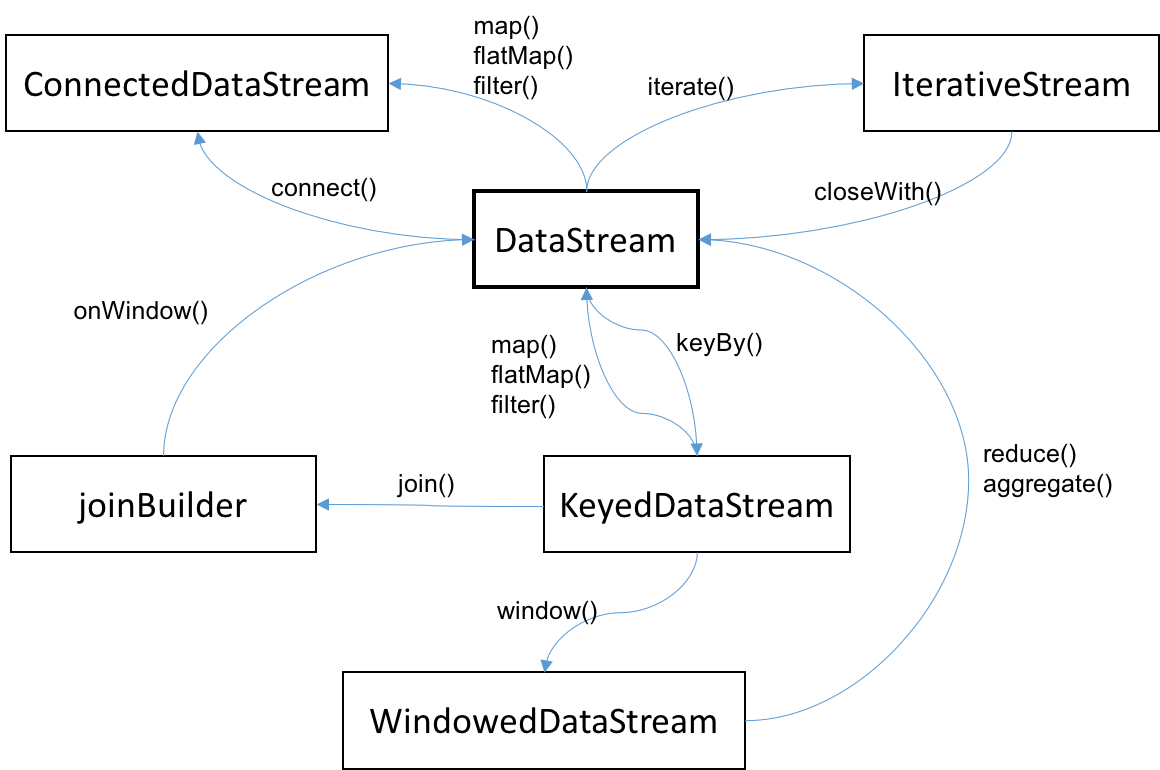
\includegraphics[scale=0.55]{images/flink_model}}
   \caption{Flink computing model}
   \label{fig:flink_model}
  \end{center}
\end{figure}

\begin{itemize}
\item A KeyedDataStream represents a data stream where elements are evaluated as ``grouped" by a specified key. 
\item In a WindowedDataStream, records in the stream are organized into groups by the key, and per group, they are windowed together by the windowing. A WindowedDataStream is always created from a KeyedDataStream that assigns records to groups.
\item The ConnectedDataStream is a way to share state between two tuple-at-a-time operations. It can be through of as executing two \texttt{map} (or \texttt{flatMap}) operations in the same object.
\end{itemize}

The transformations between different states of DataStream could be shown as Figure~\ref{fig:flink_model}. 

Similar to Storm, Flink supports cycle in the graph model. Flink supports the iterations in native platform by defining a step function and embedding it into a special iteration operator. There are two variants of this operator: \texttt{Iterate} and \texttt{Delta Iterate}. Both operators repeatedly invoke the step function on the current iteration state until a certain termination condition is reached.

\section{Apache Spark}
\label{section:spark}

Apache Spark is currently the most active open source large-scale data processing framework used in many enterprises across the world. It was originally developed in 2009 in UC Berkeley's AMPLab, and open sourced in 2010 as an Apache project. Compared to other big data and MapReduce technologies like Hadoop and Storm, Spark has several advantages. 

Spark is very easy to use by providing APIs in Scala, Java, Python and R languages. Moreover, there are more than 80 high-level built-in operators.  In the case of implementing a simple WordCount application, all the execution logic code could be written in one line with Spark' Scala API.

Spark powers a stack of libraries including SQL and DataFrames, MLlib for machine learning, GraphX, and Spark Streaming. You can combine these libraries seamlessly in the same application. It can access diverse data sources including HDFS, Cassandra, HBase, and S3.

Spark achieves much better performance than Hadoop MapReduce mainly because Spark supports in-memory computing. By using RDDs which will be discussed in \cref{subsection:rdd}, intermediate results could be kept in memory and reused for further performing functions thereafter, as opposed to being written to hard disk. 

\subsection{ Resilient Distributed Dataset(RDD)}
\label{subsection:rdd}
\textbf{R}esilient \textbf{D}istributed \textbf{D}ataset(RDD) is a fault-tolerant abstraction of read-only collection of elements partitioned across the distributed computer nodes in memory which can be operated on in parallel. To achieve fault-tolerant property, RDDs can only be created through deterministic operations on either (1) data in stable storage, or (2) other RDDs \cite{zaharia2012resilient}. An RDD could keep all information about how it was derived from other datasets to compute its partitions from data in table storage. Therefore, RDDs are fault tolerance because they could be reconstructed from a failure with these kept information. 

RDD supports two different kinds of operations, transformation and action. When a transformation operation is called on a RDD object, a new RDD returned and the original RDD remains the same. For example, map is a transformation that passes each element in RDD through a function and returns a new RDD representing the results. Some of the transformation operations are \texttt{map}, \texttt{filter}, \texttt{flatMap}, \texttt{groupByKey}, and \texttt{reduceByKey}. 

An action returns a value to the driver program after running a computation on the RDD. One representative action is \texttt{reduce} that aggregates all the elements of the RDD using some function and returns the final result to the driver program. Other actions include \texttt{collect}, \texttt{count}, and \texttt{save}.

By default, each transformed RDD is recomputed each time you run an action on it. However, by caching RDD in memory, allowing it to be reused efficiently across parallel operations. The recomputation of cached RDD is avoided and a significant amount of disk I/O could be reduced. Especially in the case of looping jobs, the performance would be improved. In Spark, users can manually specify if working sets are cached or not. The runtime engine would manage low-level caching mechanism like how to distribute cache blocks.

\subsection{Computational Model}

\begin{figure}
  \begin{center}
  \subfigure{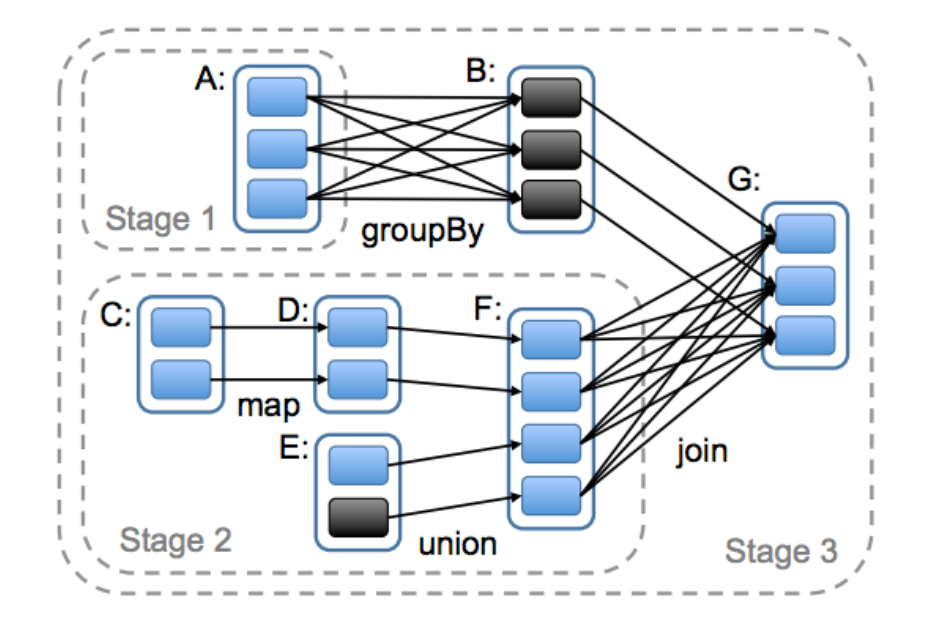
\includegraphics[scale=0.5]{images/spark_stage}}
   \caption{Spark job stages\cite{zaharia2012resilient}}
   \label{fig:spark_stage}
  \end{center}
\end{figure}

The execution engine of Spark supports lazy evaluation. When transformations applied to an RDD, the execution engine doesn't do any computation, but remember the transformations. The transformations are only computed when an action requires a result to be returned to the driver program. This design enables Spark to run more efficiently. For example, when a reduce operation is performed on a dataset created through transformation map, only the result of the reduce is returned to the driver program, rather than the larger mapped dataset.

Spark has an advanced directed acyclic graph (DAG) execution engine that implements stage-oriented scheduling. The are two main differences between the computational model of Spark Streaming and other two systems. First, the computing unit in Spark Streaming is a dataset. While in Storm and Flink, it is one single record tuple. The other difference is each node in DAG is a stage which contains as many pipelined transformations with narrow dependencies as possible. Whenever a user runs an action (e.g., count or save) on an RDD, the scheduler examines that RDD's lineage graph to build a DAG of stages to execute, as illustrated in Figure~\ref{fig:spark_stage}. The boundaries of the stages are the shuffle operations required for wide dependencies, or any already computed partitions that can short-circuit the computation of a parent RDD \cite{zaharia2012resilient}. The execution engine executes each stage in computer nodes that perform on distributed partitions of RDD in parallel. Different with Flink's pipeline execution model, Spark does not execute multi stages simultaneously \cite{shi2015clash}. In the DAG, tasks of a stage wouldn't start until all its dependencies are done. 


\subsection{Spark Streaming}

Spark Streaming is an extension of the core Spark API that enables scalable, high-throughput, fault-tolerant stream processing of live data streams. Spark Streaming receives live input data streams and divides the data into micro batches, which are then processed by the Spark engine to generate the final stream of results in batches. Each batch is processed in a Spark batch processing job. The model of Spark Streaming is different from that of Storm and Flink, which process stream records one by one. In Spark Streaming, data streams are divided according to a configurable interval. Divided data stream is abstracted as discretized stream or DStream, which represents a continuous stream of data. 

DStreams can be created either from input data streams from sources such as Kafka, Flume, and Kinesis, or by applying high-level operations on other DStreams. Internally, a DStream is represented as a sequence of micro RDDs. After applied transformations or actions on a DStream, a new DStream or result values would be get which can be pushed out to filesystems, databases, and live dashboards.

\begin{figure}
  \begin{center}
  \subfigure{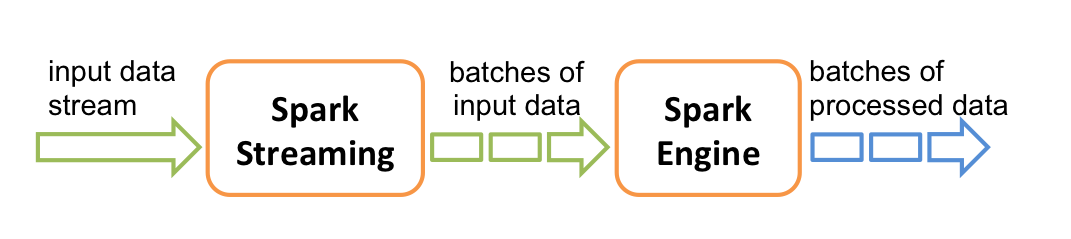
\includegraphics[scale=0.65]{images/spark_stream}}
   \caption{Spark Streaming Model}
   \label{fig:spark_stream}
  \end{center}
\end{figure}

\section{Other Stream Processing Systems}
\subsection{Apache Samza}
\begin{figure}
  \begin{center}
  \subfigure{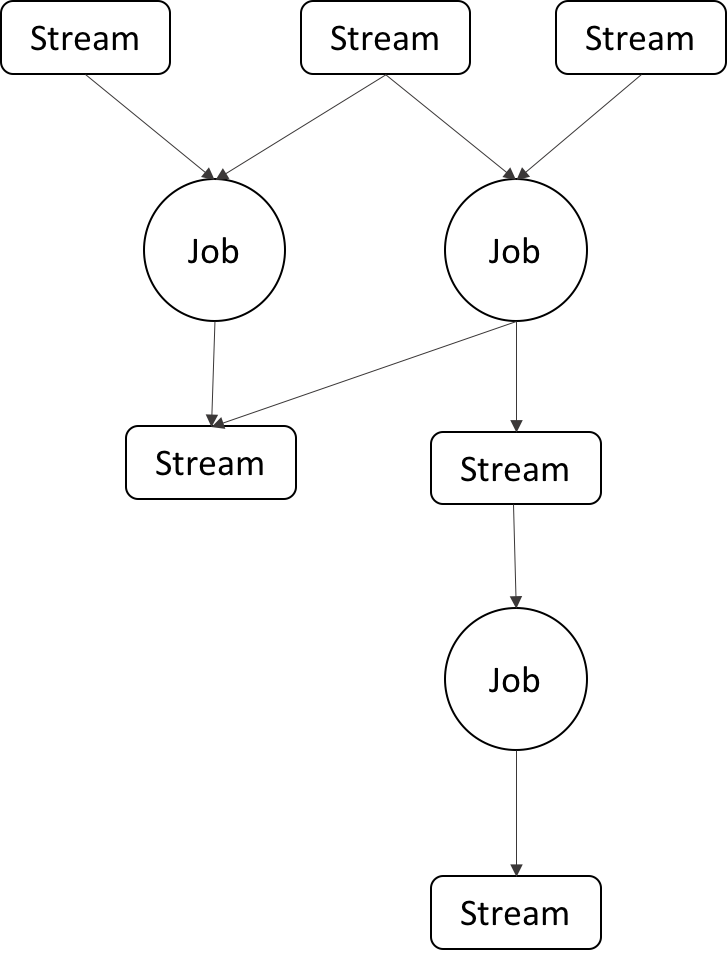
\includegraphics[scale=0.5]{images/samza_dataflow}}
   \caption{Samza DataFlow Graph}
   \label{fig:smaza_dataflow}
  \end{center}
\end{figure}

Apache Samza is a top-level project of Apache Software Foundation which open sourced by LinkedIn to solve stream processing requirements. It's been in production at LinkedIn for several years and currently runs on hundreds of machines. 

A Samza application is constructed out of streams and jobs. A stream is composed of immutable sequences of messages of a similar type or category.  A Samza job is code that performs a logical transformation on a set of input streams to append output messages to set of output streams. In order to scale the throughput of the stream processor, streams are broken into partitions and jobs are divided into smaller units of execution called tasks. Each task consumes data from one or more partitions for each of the job's input streams. Multiple jobs could be composed together to create a dataflow graph, where the nodes are streams containing data, and the edges are jobs performing transformations. 


Except streams and jobs, Samza uses YARN as execution layer. The architecture of Samza follows a similar pattern to Hadoop which could be shown as Figure~\ref{fig:smaza_architecture}.

\begin{figure}
  \begin{center}
  \subfigure{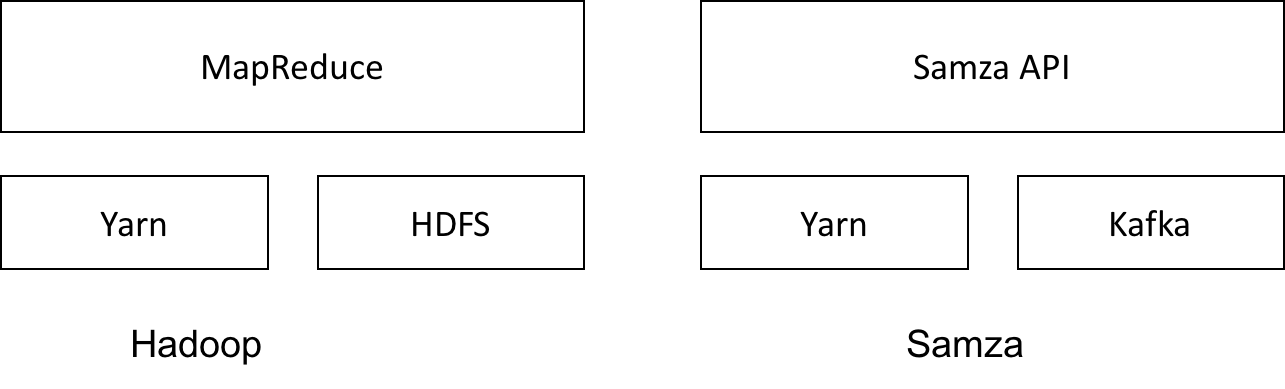
\includegraphics[scale=0.5]{images/samza_architecture}}
   \caption{Samza and Hadoop architecture}
   \label{fig:smaza_architecture}
  \end{center}
\end{figure}

\subsection{Apache S4}
S4 is another open source distributed, scalable, fault-tolerant, stream data processing platform released by Yahoo.

In S4, a stream is defined as a sequence of events of the form (\textbf{K,V}) where \textbf{K} is the key of record tuple, and V is the corresponding value. Processing Element(PE) is the basis computational unit that consume streams and applies computational logic. After takes in an event, a PE either emits one or more events which may be consumed by other PEs or publishes results\cite{neumeyer2010s4}.

S4 makes sure that two events with the same key end up being processed on the same machine. Crucial to the scalability of S4 is the idea that every instance of a processing element handles only one key. The size of an S4 cluster corresponds to the number of logical partitions. 
 
\clearpage